%arara: lualatex: { branch: developer, interaction: errorstopmode,
%arara: --> shell: yes, synctex: yes }
%arara: makeglossaries if found('aux', '@istfilename')
%arara: biber: { options: [ '--wraplines' ] }

% \DocumentMetadata{testphase=phase-III}
% \DocumentMetadata{lang=es-MX}

% NOTA: [<+->] se usa comio overlay para hacer que los bullets aparezcan uno por uno.

\documentclass[spanish,mexico]{scrartcl}
% \listfiles

\KOMAoptions{abstract=true}
\usepackage[spanish,mexico]{babel}


\usepackage{fontspec}
    \setmainfont{TeX Gyre Pagella}
    \setsansfont{TeX Gyre Heros}

\usepackage{csquotes}
% \MakeAutoQuote{"}{"}

\usepackage{microtype}
\usepackage{tabularray}
\UseTblrLibrary{booktabs}
\UseTblrLibrary{siunitx}

\usepackage{siunitx}
\sisetup{separate-uncertainty,per-mode=symbol,detect-all,range-phrase=--}
\DeclareSIUnit{\angstrom}{\textup{\AA}}
\usepackage{chemmacros}
\usepackage[eps,librsvg]{chemobabel}
\usepackage{glossaries}
    \makeglossaries{}

\usepackage[style=science,backend=biber,url=false]{biblatex}
    \addbibresource[location=remote]{http://127.0.0.1:23119/better-bibtex/export/library?/1/library.biblatex}

\usepackage[skins]{tcolorbox}
\usepackage{paralist}
\usepackage{cleveref}
\usepackage{subcaption}
\usepackage[colorinlistoftodos]{todonotes}
\usepackage{newfloat}
\DeclareFloatingEnvironment[
   fileext=los,
   listname={List of Schemes},
   name=Scheme,
   placement=tbp,
   within=none % don't reset numbering
]{scheme}
\DeclareCaptionSubType{scheme}



\begin{filecontents}[force]{abreviaturas.tex}
    \newacronym{DFT}{DFT}{Teoría del funcional de la densidad \textit{(del inglés "Density Functional Theory")}}
    \newacronym{TDDFT}{TDDFT}{Teoría del funcional de la densidad tiempo-dependiente \textit{(del inglés "Time-Dependant Density Functional Theory")}}
    \newacronym{FMR}{FMR}{Rotores Moleculares Fluorescentes \textit{(Del inglés Flurescent Molecular Rotor)}}
    \newacronym{BOSCHIBA}{BOSCHIBA}{Bases de Schiff de Boro \textit{(del inglés "\textsc{Bo}ron \textsc{Schi}ff \textsc{Ba}ses")}}
    \newacronym{BODIPY}{BODIPY}{\textsc{bo}ron-\textsc{di}\textsc{py}rromethene}
    \newacronym{TICT}{TICT}{transferencia de carga intramolecular retorcida \textit{(del inglés "twsited intramolecular charge transfer")}}
    \newacronym{LE}{LE}{Local Excitado \textit{(del inglés "locally exited")}}
    \newacronym{PES}{PES}{Superficie de Energía Potencial \textit{(del inglés "Potential Energy Surface")}}
    \newacronym{NBO}{NBO}{Orbitales Naturales de Enlace \textit{(del inglés "Natural Bond Orbitals")}}
    \newacronym{ICT}{ICT}{Transferencia de Carga Intramolecular \textit{(del inglés "Intramolecular Charge Transfer")}}
    \newacronym{VEE}{VEE}{Energía de Emisión Vertical \textit{(del inglés "Vertical Emission Energy")}}
    \newacronym{FMO}{FMO}{Orbitales Moleculares de Frontera \textit{(del inglés "Frontier Molecular Orbitals")}}
    \newacronym{HOMO}{HOMO}{Orbital Molecular de mas alta energía \textit{(del inglés "Highest Occupied Molecular Orbital")}}
    \newacronym{LUMO}{LUMO}{Orbital Molecular no ocupado de más baja energía \textit{(del inglés "Lowest Unoccupied Molecular Orbital")}}
\end{filecontents}

\begin{filecontents}[force]{comandos.tex}
    % \newcommand{\invitro}{\textit{in-vitro}}
\end{filecontents}

\begin{filecontents}[force]{quimica.tex}
    \DeclareChemReactant{BO1}{name={BO1}, short={THF}}
    \DeclareChemReactant{BO-trp}{name={triptófano}, short={BO-trp}}
    \DeclareChemReactant{BO-phe}{name={fenilalanina}, short={BO-phe}}
    \DeclareChemReactant{BO-tyr}{name={tirosina}, short={BO-tyr}}
    \DeclareChemReactant{BO-gly}{name={glicina}, short={BO-gly}}
    \NewChemLatin\invitro{in vitro}
    \NewChemLatin\insilico{in silico}
    \DeclareChemTranslation{scheme-name}{spanish}{Esquema}
    \DeclareChemTranslation{scheme-list}{spanish}{Lista de esquemas}
    \DeclareChemTranslation{scheme}{spanish}{esquema}
    \DeclareChemTranslation{schemes}{spanish}{esquemas}
    \DeclareChemTranslation{Scheme}{spanish}{Esquema}
    \DeclareChemTranslation{Schemes}{spanish}{Esquemas}
    \renewcommand{\schemename}{Esquema}
\end{filecontents}

%% LaTeX2e file `abreviaturas.tex'
%% generated by the `filecontents' environment
%% from source `PEAG-Protocolo_maestria' on 2023/09/17.
%%
    \newacronym{DFT}{DFT}{Teoría del funcional de la densidad \textit{(del inglés "Density Functional Theory")}}
    \newacronym{TDDFT}{TDDFT}{Teoría del funcional de la densidad tiempo-dependiente \textit{(del inglés "Time-Dependant Density Functional Theory")}}
    \newacronym{FMR}{FMR}{Rotores Moleculares Fluorescentes \textit{(Del inglés Flurescent Molecular Rotor)}}
    \newacronym{BOSCHIBA}{BOSCHIBA}{Bases de Schiff de Boro \textit{(del inglés "\textsc{Bo}ron \textsc{Schi}ff \textsc{Ba}ses")}}
    \newacronym{BODIPY}{BODIPY}{\textsc{bo}ron-\textsc{di}\textsc{py}rromethene}
    \newacronym{TICT}{TICT}{transferencia de carga intramolecular retorcida \textit{(del inglés "twsited intramolecular charge transfer")}}
    \newacronym{LE}{LE}{local excitado \textit{(del inglés "locally exited")}}

%% LaTeX2e file `comandos.tex'
%% generated by the `filecontents' environment
%% from source `Presentación-Protocolo-Maestria-PEAG' on 2023/11/14.
%%
    % \newcommand{\invitro}{\textit{in-vitro}}
    \newcommand\scan{\(\text{r}^{2}\text{SCAN-3c}\)}


%% LaTeX2e file `quimica.tex'
%% generated by the `filecontents' environment
%% from source `PEAG-Protocolo_maestria' on 2023/09/17.
%%
    \DeclareChemReactant{BO1}{name={BO1}, short={THF}}
    \DeclareChemReactant{BO-trp}{name={triptófano}, short={BO-trp}}
    \DeclareChemReactant{BO-phe}{name={fenilalanina}, short={BO-phe}}
    \DeclareChemReactant{BO-tyr}{name={tirosina}, short={BO-tyr}}
    \DeclareChemReactant{BO-gly}{name={glicina}, short={BO-gly}}
    \NewChemLatin\invitro{in vitro}
    \NewChemLatin\insilico{in silico}
    \DeclareChemTranslation{scheme-name}{spanish}{Esquema}
    \DeclareChemTranslation{scheme-list}{spanish}{Lista de esquemas}
    \DeclareChemTranslation{scheme}{spanish}{esquema}
    \DeclareChemTranslation{schemes}{spanish}{esquemas}
    \DeclareChemTranslation{Scheme}{spanish}{Esquema}
    \DeclareChemTranslation{Schemes}{spanish}{Esquemas}
    \renewcommand{\schemename}{Esquema}


\title{Síntesis sustentable, caracterización química-fotofísica, y por {DFT} de {BOSCHIBA} derivadas de aminoácidos y su aplicación in vitro}
\subject{Protocolo de tesis de maestría}
\date{\today}
\author{Pablo E. Alanis González}
\publishers{Universidad Autónoma de Nuevo León, División de Posgrado}

\begin{document}
\maketitle

\begin{abstract}
    Se sintetizarán una serie de \gls{BOSCHIBA} derivadas de \reactant{BO-trp}, \reactant{BO-phe}, \reactant{BO-tyr} y \reactant{BO-gly}. Se caracterizarán por métodos espectroscópicos. Se realizarán cálculos \insilico{} por medio de \gls{DFT} y \gls{TDDFT} para estudiar las propiedades fotofísicas de los compuestos y comprobar los mecanismos involucrados en el efecto supresor de la luminisencia en dichos compuestos así como estudios de topológicos sobre estos. A su vez, se realizarán estudios de citotoxicidad y tinción \invitro{} para determinar su actividad biológica de los compuestos.
\end{abstract}

\tableofcontents
% \listoffigures
% \listoftables
% \listofschemes

\section{Introducción}

Recientemente, se ha acrecentado el interés por los compuestos fluorescentes de boro debido a su amplio campo de aplicaciones; \autocite{ibarra-rodriguezOrganoboronSchiffBases2019} ya sea en sensores, como en tintas de seguridad, o bien los \gls{BODIPY} comercialmente disponibles utilizados como agentes para la tinción celular, ER-Tracker™ Green y ER-Tracker™ Red (ver \cref{ER-Trackers}).

\begin{scheme}
\centering
\begin{subscheme}{0.45\linewidth}
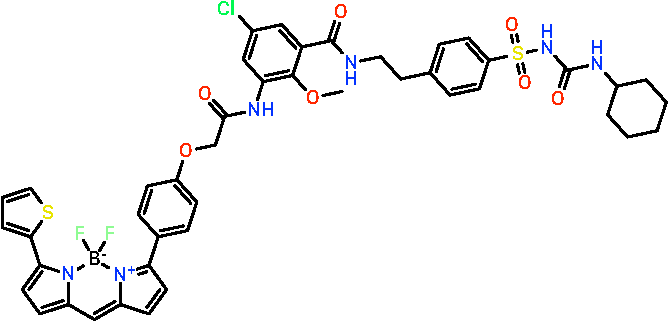
\includegraphics[width=\linewidth]{ER-Tracker_Blue.pdf}
\caption{ER-Tracker™ Blue}
\label{ER-Tracker_Blue}
\end{subscheme}
\hfill
\begin{subscheme}{0.45\linewidth}
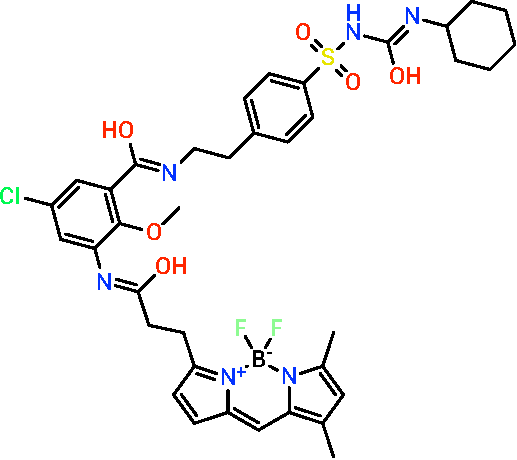
\includegraphics[width=\linewidth]{ER-Tracker_Green.pdf}
\caption{ER-Tracker™ Green}
\label{ER-Tracker_Green}
\end{subscheme}
\caption{Los ER-Tracker™ Green y ER-Tracker™ Red de Thermo Fischer Scientific™ son \gls{BODIPY} comerciales utilizados como agentes para la tinción celular.}
\label{ER-Trackers}
\end{scheme}

Los \gls{FMR} son fluoróforos sensibles a la viscosidad que presentan una rotación libre que se vuelven fluorescentes, o en su defecto, aumentan la fluorescencia solo si su rotación se ve restringida.\todo{Citar} Algunas interacciones de carácter intramolecular para detener la rotación de los \gls{FMR} son \begin{inparaenum}[i.]
    \item formar interacciones de hidrógeno,\autocite{wuMultistageRotationalSpeed2018}
    \item a través del impedimento estérico,\autocite{faulknerAllostericRegulationRotational2016} o
    \item por la formación de complejos estables con iones metálicos.\autocite{yadavViscochromicMechanochromicUnsymmetrical2019}
\end{inparaenum}

Se ha determinado que la polarización del solvente y la viscosidad del mismo afectan considerablemente la fluorescencia de los \gls{FMR}. Esto es porque se limita la tasa de formación del complejo \gls{TICT}, el cual se de-exita de forma \emph{no-radiativa,} y se promueve la formación del complejo \gls{LE}, el cual fluórese. El efecto que tiene la polarización del solvente, aunque se sabe que es importante, no se ha logrado elucidar de forma aislada a la viscosidad.\cite{haidekkerEffectsSolventPolarity2005}

Diferentes estrategias para el diseño de \gls{FMR} se han propuesto para realizar sensores de viscosidad altamente sensibles, por ejemplo, incorporando grupos rotacionales asimétricos,\autocite{leePyrrolicMolecularRotors2016} rotadores con alta capacidad rotacional,\autocite{karpenkoPushPullDioxaborine2016} variación de puentes π-conjugados \emph{push-pull},\autocite{karpenkoPushPullDioxaborine2016} la aplicación de rotadores di- o trímeros,\autocite{kimballBODIPYBODIPYDyad2015} y la introducción de dos rotadores con diferentes capacidades rotacionales y electrondonantes.\autocite{rautTriazinebasedBODIPYTrimer2016}

Por lo que, obtener tanto una alta eficiencia de fluorescencia como un contraste fluorescente simultáneamente es muy difícil, debido a que, en muchos casos, las moléculas de alto rendimiento cuántico tienen una capacidad de contraste deficiente. 
El rendimiento cuántico y el contraste de fluorescencia de los \gls{FMR} están inversamente correlacionados, una relación llamada "intensidad de fluorescencia---contraste".\autocite{leeFrontCoverFluorescent2018}

En la actualidad existe una amplia variedad de \gls{FMR} derivados de compuestos de boro, donde los \gls{BODIPY} y los dioxaborinos son los protagonistas debido a su elevado rendimiento cuántico, sin embargo, muestran algunas desventajas como la síntesis en varias etapas, condiciones de atmósfera anhidra y, en muchas ocasiones, una capacidad de contraste baja, aumentando escasamente el rendimiento cuántico del valor inicial.\autocite{karpenkoPushPullDioxaborine2016,guptaBodipyBasedFluorescent2016,liBODIPYBasedTwoPhotonFluorescent2018,kimBorondifluorideComplexesHemicurcuminoids2016}

Recientemente, nuestro grupo de trabajo ha informado sobre la síntesis de \gls{BOSCHIBA} y su uso como \gls{FMR} en la detección de viscosidad y la bioimagen de células.\autocite{ibarra-rodriguezFluorescentMolecularRotors2017} Los resultados encontrados indican que los \gls{BOSCHIBA} pueden aumentar hasta 34 veces su valor de rendimiento cuántico en medios de alta viscosidad, sin embargo, a pesar de teñir selectivamente el citoplasma en las células de melanoma, presentaron un bajo teñido atribuido principalmente a la baja solubilidad de los compuestos.

Para lograr mejorar el contraste de fluorescencia y la bioimagen celular, se diseñó una serie de \gls{BOSCHIBA} derivados de aminoácidos (ver \cref{sch:marcha}), donde las moléculas presentan rotación libre a través del anillo fenilborónico, y el aminoácido podría dar una mayor compatibilidad y solubilidad en medios celulares. Los compuestos de boro fluorescentes \textbf{1-4} se obtuvieron por irradiación ultrasónica en combinación con una reacción multicomponente con altos rendimientos químicos (\qty{>90}{\percent}) y un tiempo de reacción corto de \qty{20}{\minute} a \qty{50}{\degreeCelsius}. Este método resulta más eficiente y rápido en comparación con moléculas similares reportadas en la literatura.

\begin{scheme}
    \centering
    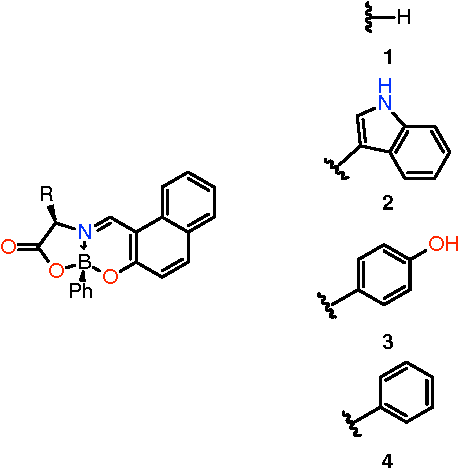
\includegraphics[width=0.5\linewidth]{Marcha.pdf}
    \caption{Compuestos que se sintetizarán en esta investigación.}
    \label{sch:marcha}
\end{scheme}

Todos los compuestos fueron caracterizados completamente, tanto estructural como fotofísicamente. Las estructuras cristalinas obtenidas para los compuestos \reactant{BO-tyr} y \reactant{BO-trp} muestran átomos de boro tetracoordinados con geometría tetraédrica ligeramente distorsionada y la formación de dos heterociclos fusionados de cinco y seis miembros debido a la coordinación N→B (ver \cref{sch:estructuras}). Las longitudes N→B, \reactant{BO-tyr} de \qty{1.569}{\angstrom} y para \reactant{BO-trp} \qty{1.566}{\angstrom} sugieren una fuerte coordinación del nitrógeno con los átomos de boro porque son menores que la distancia covalente N→B estimada; esto se confirma por el carácter tetraédrico del \qty{91.33}{\percent} y \qty{93.07}{\percent}, respectivamente.

Otra evidencia confiable de la unión de coordinación N→B fue una señal ancha alrededor de \begin{experimental} \NMR{11,B} \val{5.80}; \end{experimental} para todos los compuestos, indicativo de un átomo de boro tetracoordinado. El HRMS de los compuestos de boro mostró que el pico base corresponde al pico del ion molecular, y la primera fragmentación resulta en su ligando por pérdida del segmento fenilborónico (ver ESI). \todo{Conseguir ESI}


Con el proposito de determinar la capacidad de detección de viscosidad, se midieron los espectros de fluorescencia de 1-4 en mezclas de metanol/glicerol a diferentes fracciones, donde, el compuesto 2 muestra que la intensidad de fluorescencia aumenta significativamente con un aumento de la fracción de glicerol (ver \cref{fig:fluorescencia-glicerol}), mientras que el resto de los compuestos no muestran un cambio significativo en su intensidad de fluorescencia (ver ESI).\todo{Conseguir ESI} En el medio sin glicerol, el rendimiento cuántico de 2 es menor que \qty{0.04}{\percent} y aumenta alrededor de 100 veces en alta fracción de glicerol con \qty{0.40}{\percent} de rendimiento cuántico. Hasta hoy no había un alto sensibilizador de viscosidad.

\begin{figure}
    \centering
    \missingfigure[figheight=10cm,figwidth=10cm]{Espectro de fluoresencia con diferentes viscosidades. Ya existe pero se ocupa de calidad más alta.}
    \label{fig:fluorescencia-glicerol}
    \caption{Espectro de fluoresencia del \reactant{BO-phe} con glicerol en diferentes proporciones. A mayor viscosidad se observa un aumento en la fluorescencia.}
\end{figure}

Para lograr comprender mejor las propiedades fotofísicas en solución, se desarrollaron estudios \insilico{} para las moléculas, utilizando el método \texttt{B3LYP/6-31G(d,p),} implementado en Gaussian 09. Explorando las estructuras de energía mínima de 1-4, obtenidas por \gls{PES}, el fragmento de triptófano en la molécula 2 genera una obstrucción estérica significativa en el anillo fenilborónico, causando un ángulo de torsión diédrico de \qty{73.5}{\degree}, a diferencia del resto de las estructuras (1, 3 y 4),\todo{poner con comando \texttt{reactant}} donde el fragmento de aminoácido no causa ninguna obstrucción estérica y los ángulos de torsión diédricos están cerca de \qty{55}{\degree} (ver ESI).\todo{Conseguir ESI} Además, se calcularon los \gls{NBO} para las estructuras optimizadas.
Las principales transferencias de carga en todas las moléculas se dan por N→B, O1→B y O2→B, donde, los átomos de nitrógeno y oxígenos actúan como donadores de electrones y el átomo central de boro actúa como aceptor de electrones. En el caso de las moléculas 1, 3 y 4,\todo{poner con comando \texttt{reactant}} que no tienen obstrucción estérica, se observan mayores transferencias de carga por grupos donador-aceptor debido a una mejor superposición de orbitales, en comparación con el compuesto 2 derivado del triptófano. Sin embargo, cuando el ángulo de torsión diédrico se modifica a \qty{55}{\degree} y se calculan los \gls{NBO}, se recupera la superposición óptima de orbitales y se obtienen valores de transferencia de carga similares.

En un medio de alta viscosidad, la molecula 2\todo{poner con comando \texttt{reactant}} no puede tener flexibilidad estructural o la obstrucción estérica podría suprimirse, permitiendo que la superposición orbital no se vea afectada. Este comportamiento del compuesto 2\todo{poner con comando \texttt{reactant}} podría explicar la disminución significativa del rendimiento cuántico experimental en solución y sugiere que el mecanismo de detección de viscosidad ocurre a través de la modificación de las propiedades de transferencia de carga intramolecular por la obstrucción estérica del triptófano.

Subsecuentemente, se calcularon las \gls{VEE} para el primer estado excitado, al mismo nivel de teoría. Los valores de \gls{VEE} obtenidos para 1-4\todo{poner con comando \texttt{reactant}} fueron \qtylist[list-units = bracket]{60.15;41.83;52.65;60.52}{\kilo\cal\per\mol}, respectivamente, mostrando valores de 2\todo{poner con comando \texttt{reactant}} inferiores al resto de los compuestos y coincidiendo con lo observado experimentalmente. 

En la \cref{fig:FMO} se muestran los \gls{FMO} involucrados para todos los compuestos sintetizados

\begin{figure}
    \centering
    \missingfigure[figheight=10cm,figwidth=10cm]{FMO de los compuestos. Rehacer con el funcional final}
    \label{fig:FMO}
    \caption{\gls{FMO} de los compuestos sintetizados}
\end{figure}

HOMO for 2 shows an electronic delocalization on the amino acid fragment and outside the fluorophore, unlike the rest of structures, where the HOMO shows an electronic delocalization across the naphthyl group and the new rings formed with boron atom. The LUMOs of all molecules are completely delocalized across the naphthyl and boron rings, without influence of the different amino acids. However, exploring the HOMO-1 it has similar electronic delocalization distribution that rest of compounds (see ESI), this behaviour could also explain the significant decrease of experimental quantum yield in the molecule derived from tryptophan and suggest HOMO-LUMO transition is responsible for fluorescence, nevertheless, even though HOMO-LUMO of 2 have highest energy value, the energy of these orbitals being the closest, suggesting greater mobility of the π electrons in conjugated system and better molecular stability.

El \gls{HOMO} para el compuesto 2, muestra deslocalización en el fragmento de aminoacido fuera del fluoróforo 

\section{Antecedentes}\todo{Hacer!}
\section{Análisis crítico de los antecedentes}\todo{Hacer!}
\section{Aporte científico}\todo{Hacer!}
\section{Hipótesis}\todo{Hacer!}
\section{Objetivos}\todo{Hacer!}
\subsection{Objetivo general}\todo{Hacer!}
\subsection{Objetivos específicos}\todo{Hacer!}
\section{Metodología}\todo{Hacer!}
\subsection{Síntesis}\todo{Hacer!}
\subsection{Determinación de propiedades ópticas}\todo{Hacer!}
\subsection{Determinación de citotoxicidad}\todo{Hacer!}
\subsection{Modelado molecular}\todo{Hacer!}
\subsubsection{Selección del funcional}\todo{Hacer!}
\subsubsection{Optimización}\todo{Hacer!}
\subsubsection{Obtención de espectro de emisión}\todo{Hacer!}
\section{Residuos}\todo{Hacer!}
\section{Análisis de costos}\todo{Hacer!}
\section{Procedimiento experimental}\todo{Hacer!}
\section{Planificación}\todo{Hacer!}

\printreactants{}
\printglossaries{}
\printbibliography{}

\listoftodos[Pendientes]

\end{document}
